\begingroup\hyphenpenalty=10000\relax
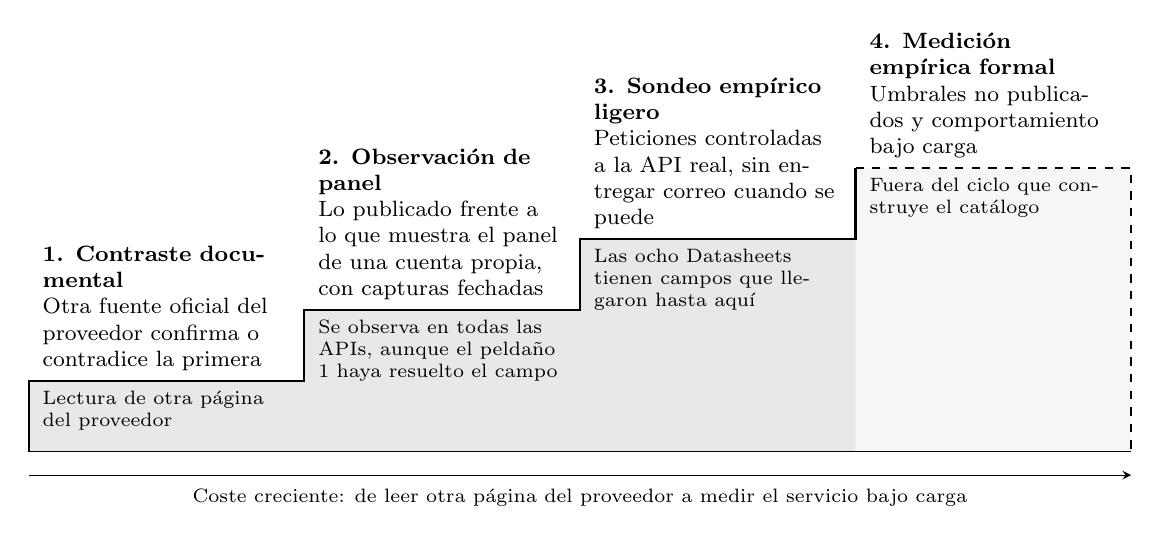
\begin{tikzpicture}[
  font=\footnotesize,
  peldano/.style={align=left, text width=31mm, anchor=south west, inner sep=2pt},
  nota/.style={align=left, text width=31mm, anchor=north west, inner sep=2pt, font=\scriptsize}
]
\fill[gray!18] (0,0) -- (0,0.9) -- (3.5,0.9) -- (3.5,1.8) -- (7,1.8) -- (7,2.7) -- (10.5,2.7) -- (10.5,0) -- cycle;
\fill[gray!7] (10.5,0) rectangle (14,3.6);
\draw[thick] (0,0) -- (0,0.9) -- (3.5,0.9) -- (3.5,1.8) -- (7,1.8) -- (7,2.7) -- (10.5,2.7) -- (10.5,3.6);
\draw[thick, dashed] (10.5,3.6) -- (14,3.6) -- (14,0);
\draw (0,0) -- (14,0);
\node[peldano] at (0.1,0.95) {\textbf{1. Contraste documental}\\ Otra fuente oficial del proveedor confirma o contradice la primera};
\node[peldano] at (3.6,1.85) {\textbf{2. Observación de panel}\\ Lo publicado frente a lo que muestra el panel de una cuenta propia, con capturas fechadas};
\node[peldano] at (7.1,2.75) {\textbf{3. Sondeo empírico ligero}\\ Peticiones controladas a la API real, sin entregar correo cuando se puede};
\node[peldano] at (10.6,3.65) {\textbf{4. Medición empírica formal}\\ Umbrales no publicados y comportamiento bajo carga};
\node[nota] at (0.1,0.85) {Lectura de otra página del proveedor};
\node[nota] at (3.6,1.75) {Se observa en todas las APIs, aunque el peldaño 1 haya resuelto el campo};
\node[nota] at (7.1,2.65) {Las ocho Datasheets tienen campos que llegaron hasta aquí};
\node[nota] at (10.6,3.55) {Fuera del ciclo que construye el catálogo};
\draw[-stealth] (0,-0.3) -- (14,-0.3);
\node[font=\scriptsize, anchor=north] at (7,-0.35) {Coste creciente: de leer otra página del proveedor a medir el servicio bajo carga};
\end{tikzpicture}
\endgroup
